\documentclass[a4paper,14pt]{extarticle} 
\usepackage[a4paper,top=1.5cm, bottom=1.5cm, left=2cm, right=1cm]{geometry}
%\usepackage[T2A]{fontenc}
%\usepackage[english, russian]{babel}
\usepackage{graphicx}
\graphicspath{{./pics/}}
\DeclareGraphicsExtensions{.pdf,.png,}

\usepackage{fontspec}
\setmainfont{Times New Roman}
\setsansfont{FreeSans}
\setmonofont{FreeMono}
\renewcommand{\baselinestretch}{1.5}
\usepackage{polyglossia}
\setdefaultlanguage{russian}
\setotherlanguages{english,russian}
\usepackage{setspace}
\usepackage[many]{tcolorbox}
\usepackage{array}

\begin{document}
    \begin{center}
        \thispagestyle{empty}
        \begin{singlespace}
        ФЕДЕРАЛЬНОЕ АГЕНТСТВО СВЯЗИ

        ФЕДЕРАЛЬНОЕ ГОСУДАРСТВЕННОЕ БЮДЖЕТНОЕ ОБРАЗОВАТЕЛЬНОЕ

        УЧРЕЖДЕНИЕ ВЫСШЕГО ОБРАЗОВАНИЯ

        «САНКТ-ПЕТЕРБУРГСКИЙ ГОСУДАРСТВЕННЫЙ УНИВЕРСИТЕТ ТЕЛЕКОММУНИКАЦИЙ ИМ. ПРОФ. М.А. БОНЧ-БРУЕВИЧА»

        (СПбГУТ)
        \end{singlespace}
        \vspace{-1ex}
        \rule{\textwidth}{0.4pt}
        \vspace{-5ex}

        \vspace{100px}
        \textbf{Лабораторная работа №3}\\
        Исследование свойств модели резисторного касакада с общим колектором в частотной и временной областях на ПК

    \vspace{100px}
    \end{center}
    \vspace{4ex}
    \begin{flushright}
    \parbox{12 cm}{
    \begin{flushleft}
        Выполнила бригада:\\
        Группа ИКТЗ-83\\
        \underline{Громов А.А., Миколаени М.С., Мазеин Д.С.} \hfill \rule[-0.85ex]{0.09\textwidth}{0.6pt}\\
        \vspace{-1ex}
        \footnotesize \textit{ (Ф.И.О., № группы) \hfill (подпись)} \normalsize


    \end{flushleft}
    }
    \end{flushright}
    \begin{center}
        \vfill
        Санкт-Петербург

        2020

    \end{center}
    \newpage

    \textbf{Цель работы:} Изучить свойства усилительного каскада с общим коллектором (ОК) в режиме малого сигнала. Выполнить анализ в частотной и временной областях. Исследовать свойства каскада при изменении сопротивлений источника сигнала, нагрузки и элементов схемы. Определить входное и выходное сопротивления каскада.

    \textbf{Пункт 1:}
    \begin{center}
        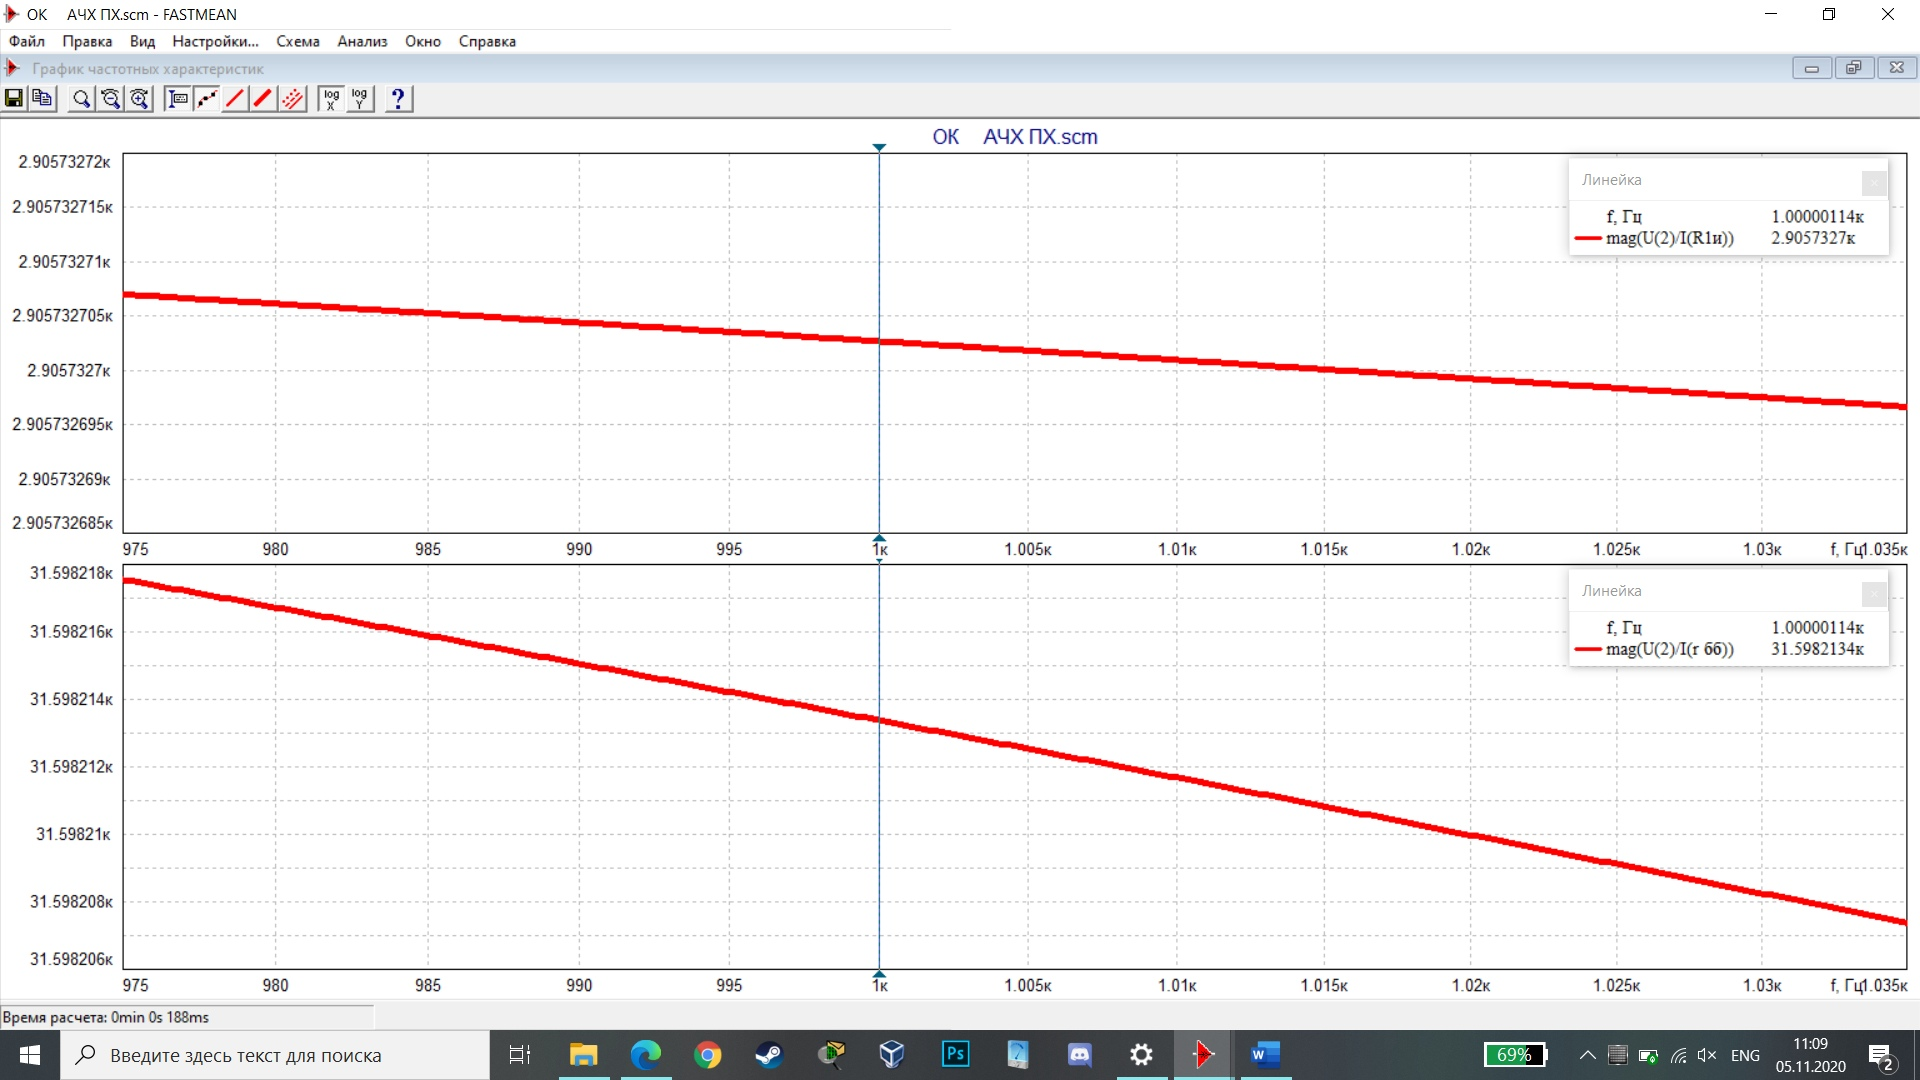
\includegraphics[scale=0.25]{1.jpg}
    \end{center}
    Окно измерения входного сопротивления 

    \begin{tabular}{ |c|c| }
        \hline
        Измерение & Величина входного сопротивления, КОм\\
        \hline
        с учётом сопротивления Rб & 31.6\\
        \hline
        без учёта сопротивления Rб & 2.91\\
        \hline
    \end{tabular}

    \newpage
    \textbf{Пункт 2:}
    \begin{center}
        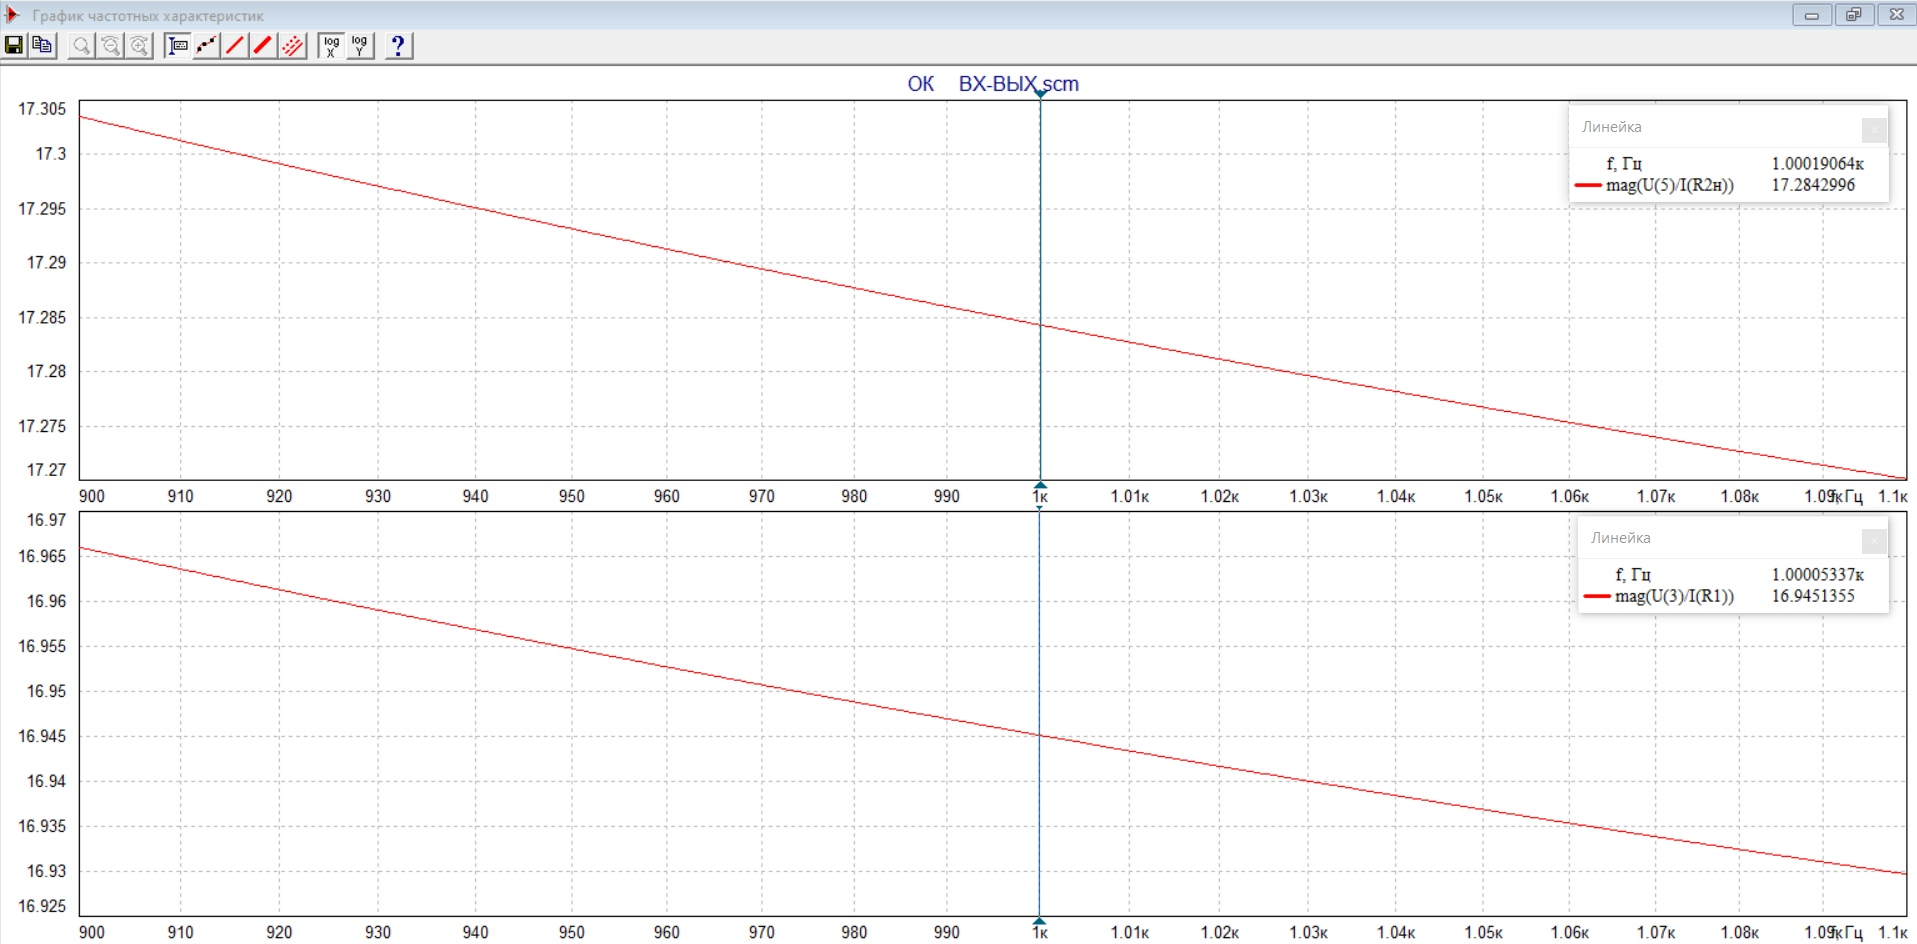
\includegraphics[scale=0.25]{2.jpg}
    \end{center}
    сопротивление 17.29\\
    сопротивление 16.95\\

    
    \textbf{Пункт 3:}
    \begin{center}
        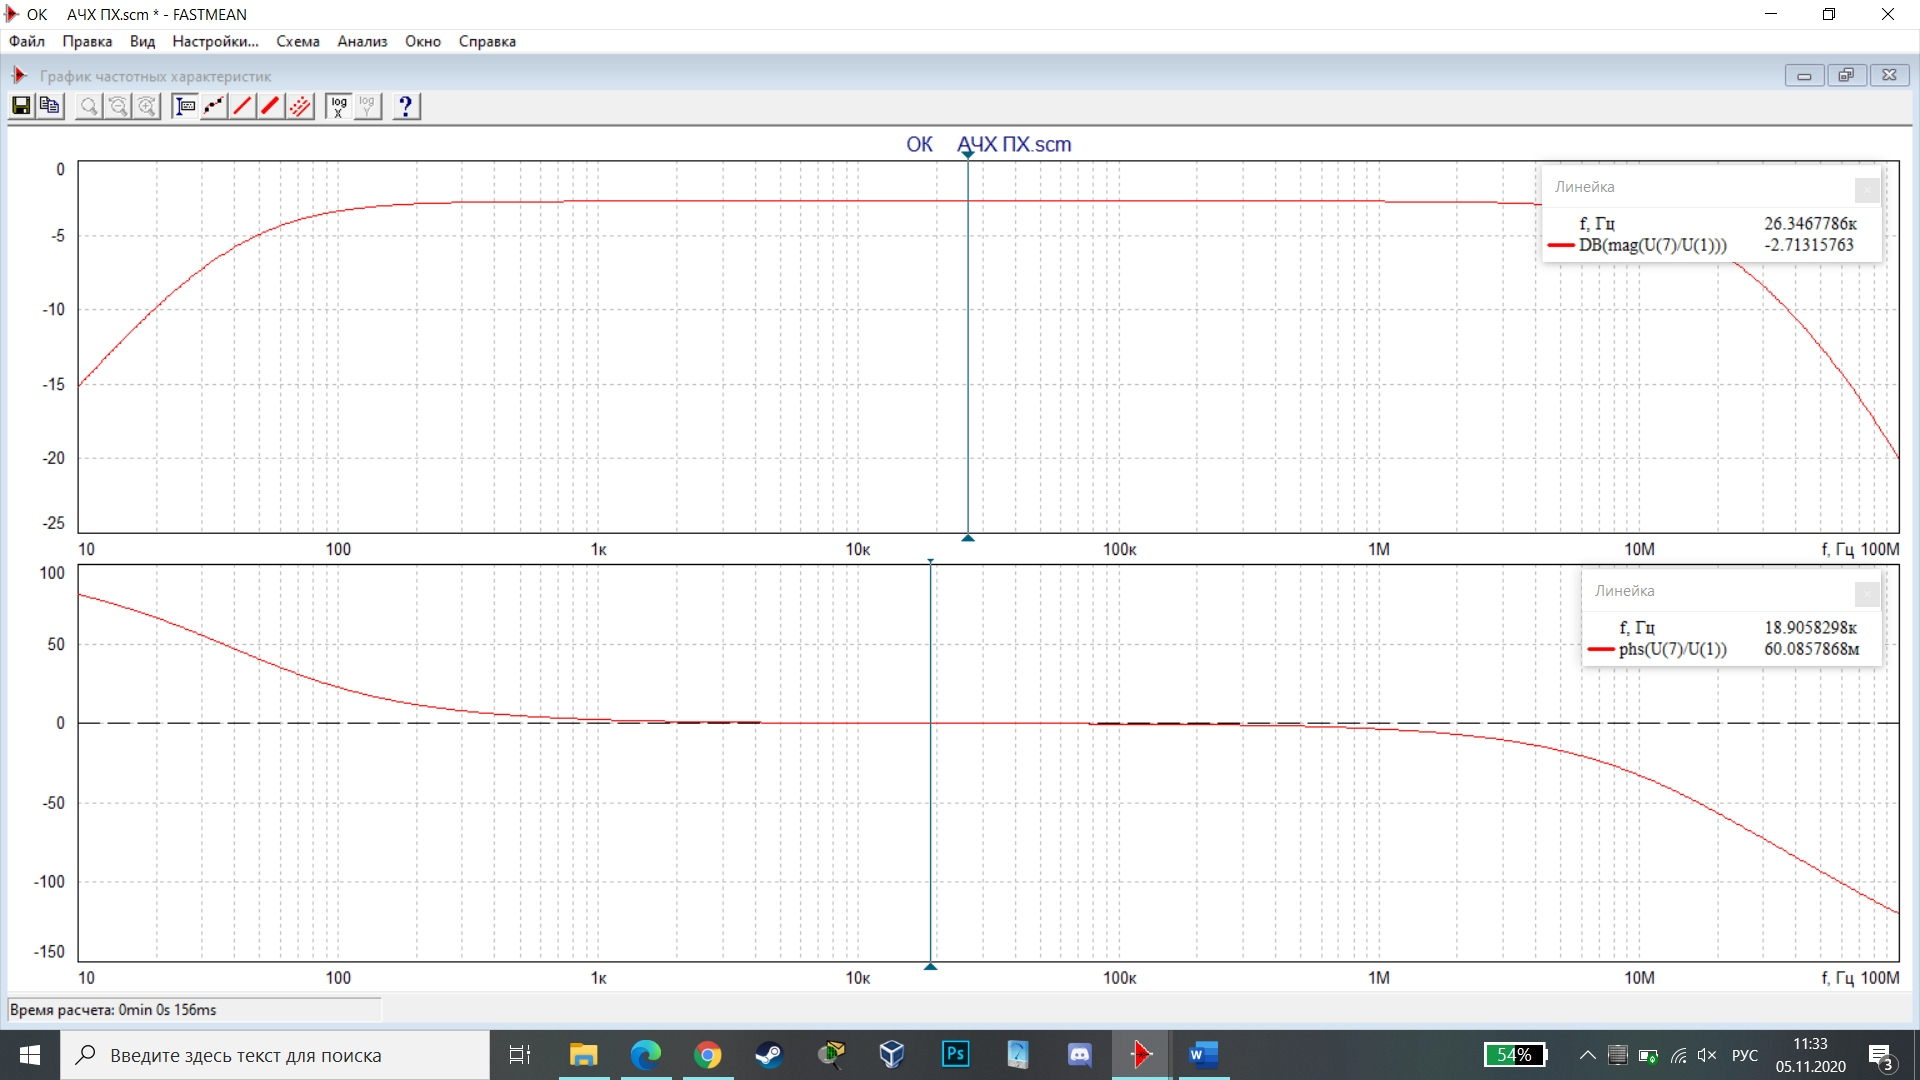
\includegraphics[scale=0.25]{3.jpg}
    \end{center}
    \begin{center}
        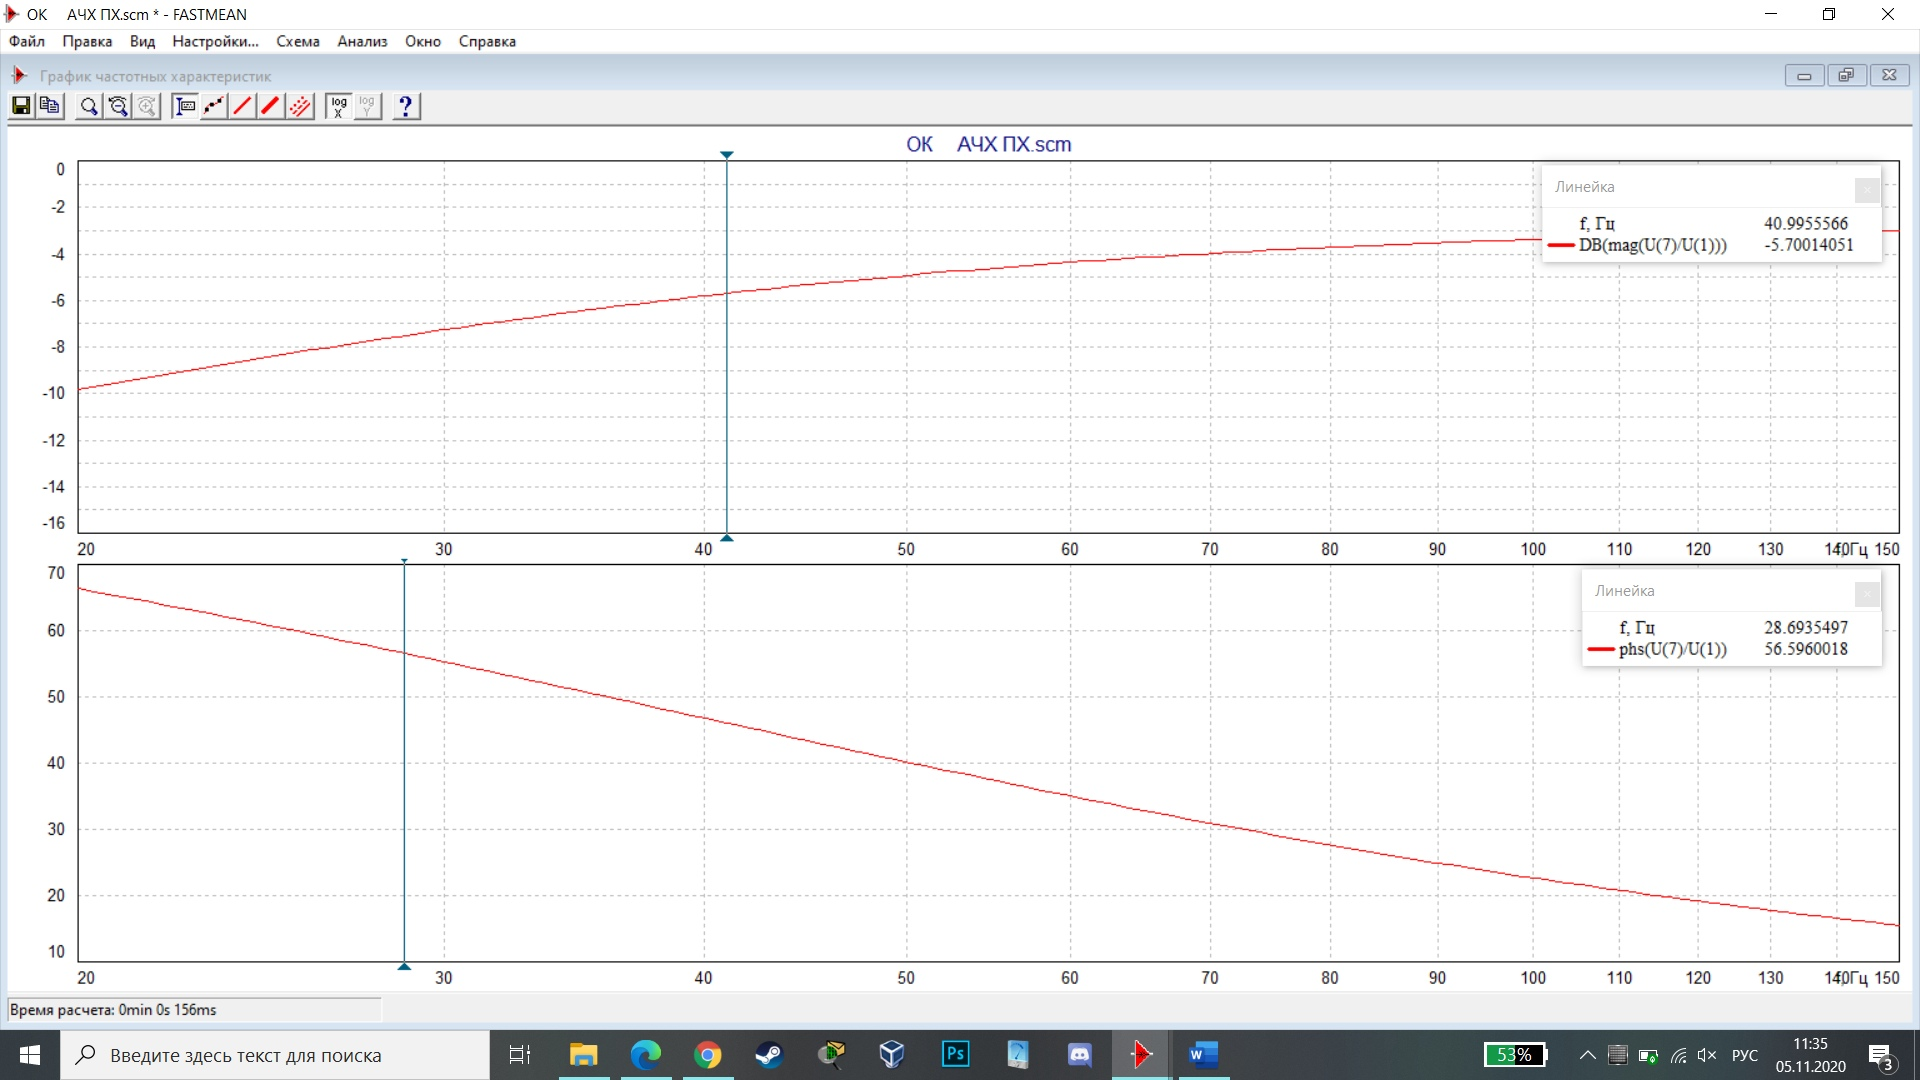
\includegraphics[scale=0.25]{4.jpg}
    \end{center}
    \begin{center}
        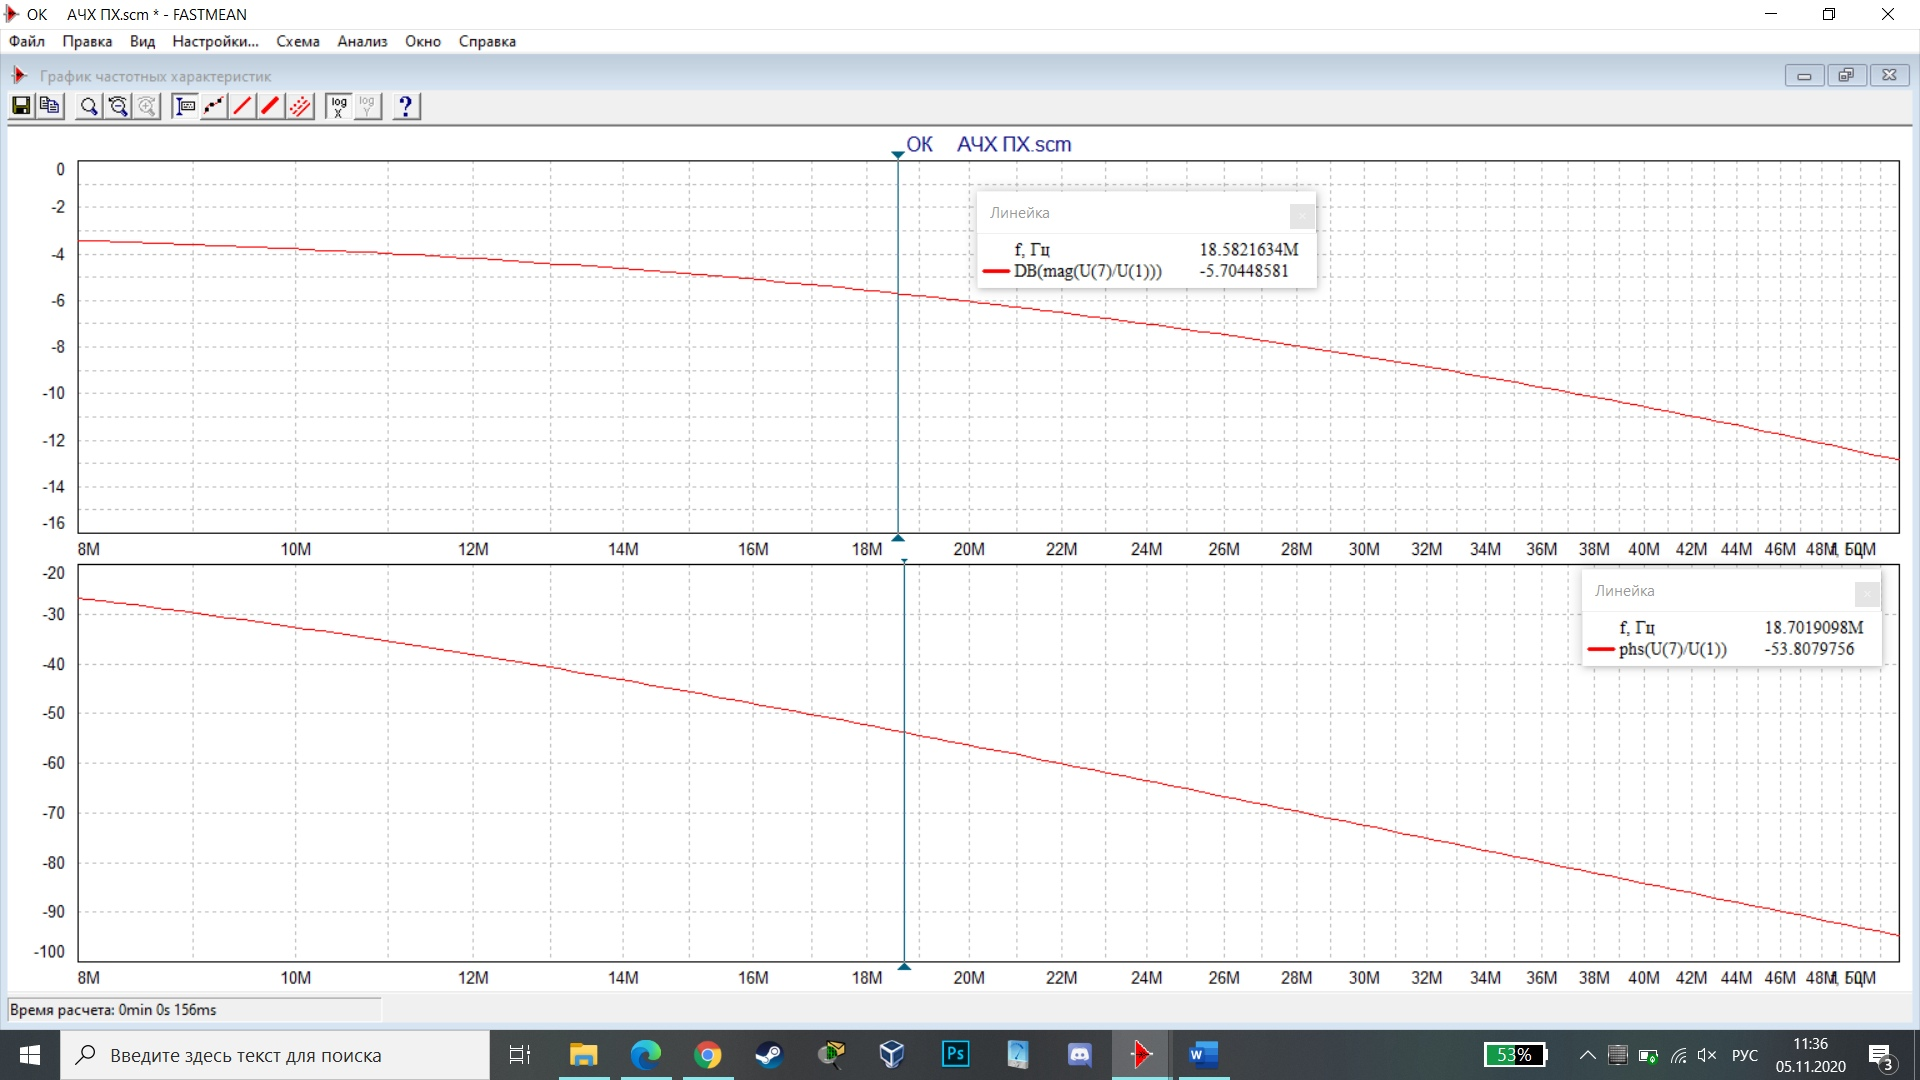
\includegraphics[scale=0.25]{5.jpg}
    \end{center}

    \begin{tabular}{ |c|c|c|c|c| }
       \hline
       Kскв, Дб & (Kскв -3), Дб&fн, Гц & fв, МГц & ∆f=fв−fн, МГц \\
       \hline 
       -2.7 & -5.7 & 41 & 18.6 & 18.56\\
       \hline
    \end{tabular}\\

    Выводы по пункту 3:

    Схема не инвертирует входной сигнал.

    У схемы с ОК рабочая полоса частот больше чем у схему с ОУ

    \newpage
    \begin{tabular}{|>{\centering}m{6cm}|>{\centering}m{5cm}|>{\centering}m{5cm}|}
        \hline 
        Время импульса & tи=25 мкс & tи=1.25 мкс\\
        \hline 
        Частота f, Гц & 20000 & 400\\
        \hline 
        Осциллограмма импульса & & \\
        \hline 
        Измеренный спад вершины импульса ∆, \% & & 27.9\\
        \hline 
        Рассчитанный спад вершины импульса ∆, \% & 0.62 & 31.4 \\
        \hline 
        Осциллограмма увеличенной области нарастания импульса & & \\
        \hline 
        Измеренное время нарастания импульса tН =t2 –t1,нс & 19.12 & \\
        \hline 
        Рассчитанное время нарастания импульса tн, нс & 18.8 & 18.8\\
        \hline 
    \end{tabular}

    \begin{tabular}{|>{\centering}p{3.5cm}|>{\centering}p{3.5cm}|>{\centering}p{3.5cm}|}
        Geometry  & Algebra &
        \tabularnewline
        \hline
         Points & Addition &
        \tabularnewline
         Spheres & Multiplication 
    \end{tabular} 
\end{document}